\documentclass{article}\usepackage[]{graphicx}\usepackage[]{color}
%% maxwidth is the original width if it is less than linewidth
%% otherwise use linewidth (to make sure the graphics do not exceed the margin)
\makeatletter
\def\maxwidth{ %
  \ifdim\Gin@nat@width>\linewidth
    \linewidth
  \else
    \Gin@nat@width
  \fi
}
\makeatother

\definecolor{fgcolor}{rgb}{0.345, 0.345, 0.345}
\newcommand{\hlnum}[1]{\textcolor[rgb]{0.686,0.059,0.569}{#1}}%
\newcommand{\hlstr}[1]{\textcolor[rgb]{0.192,0.494,0.8}{#1}}%
\newcommand{\hlcom}[1]{\textcolor[rgb]{0.678,0.584,0.686}{\textit{#1}}}%
\newcommand{\hlopt}[1]{\textcolor[rgb]{0,0,0}{#1}}%
\newcommand{\hlstd}[1]{\textcolor[rgb]{0.345,0.345,0.345}{#1}}%
\newcommand{\hlkwa}[1]{\textcolor[rgb]{0.161,0.373,0.58}{\textbf{#1}}}%
\newcommand{\hlkwb}[1]{\textcolor[rgb]{0.69,0.353,0.396}{#1}}%
\newcommand{\hlkwc}[1]{\textcolor[rgb]{0.333,0.667,0.333}{#1}}%
\newcommand{\hlkwd}[1]{\textcolor[rgb]{0.737,0.353,0.396}{\textbf{#1}}}%

\usepackage{framed}
\makeatletter
\newenvironment{kframe}{%
 \def\at@end@of@kframe{}%
 \ifinner\ifhmode%
  \def\at@end@of@kframe{\end{minipage}}%
  \begin{minipage}{\columnwidth}%
 \fi\fi%
 \def\FrameCommand##1{\hskip\@totalleftmargin \hskip-\fboxsep
 \colorbox{shadecolor}{##1}\hskip-\fboxsep
     % There is no \\@totalrightmargin, so:
     \hskip-\linewidth \hskip-\@totalleftmargin \hskip\columnwidth}%
 \MakeFramed {\advance\hsize-\width
   \@totalleftmargin\z@ \linewidth\hsize
   \@setminipage}}%
 {\par\unskip\endMakeFramed%
 \at@end@of@kframe}
\makeatother

\definecolor{shadecolor}{rgb}{.97, .97, .97}
\definecolor{messagecolor}{rgb}{0, 0, 0}
\definecolor{warningcolor}{rgb}{1, 0, 1}
\definecolor{errorcolor}{rgb}{1, 0, 0}
\newenvironment{knitrout}{}{} % an empty environment to be redefined in TeX

\usepackage{alltt}
\IfFileExists{upquote.sty}{\usepackage{upquote}}{}
\begin{document}
\title{Final Project: Statistical Analysis}
\author{Steven Layne}
\maketitle{}
\subsection*{Examining the relationship between manatee (Trichechus manatus) anatomy and environment and manatee death by watercraft collision.  }

INIT DATA FRAMES
\begin{knitrout}
\definecolor{shadecolor}{rgb}{0.969, 0.969, 0.969}\color{fgcolor}\begin{kframe}
\begin{alltt}
\hlstd{mortDat} \hlkwb{<-} \hlkwd{read.csv}\hlstd{(}\hlstr{"https://www.dropbox.com/s/jsfh8rq2ez0wsj8/ReformattedManateeMortalityData.csv?dl=1"}\hlstd{)} \hlcom{#Loads in mortality data }
\hlstd{cReg} \hlkwb{<-} \hlkwd{read.csv}\hlstd{(}\hlstr{"https://www.dropbox.com/s/mpxmf4qn7aelr9v/CountyRegions.csv?dl=1"}\hlstd{)} \hlcom{#Loads Classifier for Country Region}

\hlstd{b} \hlkwb{<-} \hlstd{mortDat}\hlopt{$}\hlstd{County[mortDat}\hlopt{$}\hlstd{County} \hlopt{==} \hlkwd{c}\hlstd{(cReg}\hlopt{$}\hlstd{North.West.Central[}\hlnum{1}\hlstd{])]}

\hlstd{southCentralWest} \hlkwb{<-} \hlkwd{vector}\hlstd{(}\hlkwc{length} \hlstd{=} \hlkwd{length}\hlstd{(mortDat}\hlopt{$}\hlstd{County))} \hlcom{#Holds booleans for region}
\hlstd{northWestCentral} \hlkwb{<-} \hlkwd{vector}\hlstd{(}\hlkwc{length} \hlstd{=} \hlkwd{length}\hlstd{(mortDat}\hlopt{$}\hlstd{County))} \hlcom{#Holds booleans for region}
\hlstd{northEastCentral} \hlkwb{<-} \hlkwd{vector}\hlstd{(}\hlkwc{length} \hlstd{=} \hlkwd{length}\hlstd{(mortDat}\hlopt{$}\hlstd{County))} \hlcom{#Holds booleans for region}
\hlstd{southCentralEast} \hlkwb{<-} \hlkwd{vector}\hlstd{(}\hlkwc{length} \hlstd{=} \hlkwd{length}\hlstd{(mortDat}\hlopt{$}\hlstd{County))} \hlcom{#Holds booleans for region}
\end{alltt}
\end{kframe}
\end{knitrout}
\begin{knitrout}
\definecolor{shadecolor}{rgb}{0.969, 0.969, 0.969}\color{fgcolor}\begin{kframe}
\begin{alltt}
\hlkwa{for}\hlstd{(i} \hlkwa{in} \hlnum{1}\hlopt{:}\hlkwd{length}\hlstd{(cReg}\hlopt{$}\hlstd{South.Central.West))\{}
  \hlstd{southCentralWest} \hlkwb{<-} \hlstd{(southCentralWest} \hlopt{|} \hlstd{(mortDat}\hlopt{$}\hlstd{County} \hlopt{==} \hlkwd{as.character}\hlstd{(cReg}\hlopt{$}\hlstd{South.Central.West[i])))}
\hlstd{\}}
\end{alltt}
\end{kframe}
\end{knitrout}
Places a True if County is a member of the region
\begin{knitrout}
\definecolor{shadecolor}{rgb}{0.969, 0.969, 0.969}\color{fgcolor}\begin{kframe}
\begin{alltt}
\hlkwa{for}\hlstd{(i} \hlkwa{in} \hlnum{1}\hlopt{:}\hlkwd{length}\hlstd{(cReg}\hlopt{$}\hlstd{North.West.Central))\{}
  \hlstd{northWestCentral} \hlkwb{<-} \hlstd{(northWestCentral} \hlopt{|} \hlstd{(mortDat}\hlopt{$}\hlstd{County} \hlopt{==} \hlkwd{as.character}\hlstd{(cReg}\hlopt{$}\hlstd{North.West.Central[i])))}
\hlstd{\}}
\end{alltt}
\end{kframe}
\end{knitrout}
Places a True if County is a member of the region
\begin{knitrout}
\definecolor{shadecolor}{rgb}{0.969, 0.969, 0.969}\color{fgcolor}\begin{kframe}
\begin{alltt}
\hlkwa{for}\hlstd{(i} \hlkwa{in} \hlnum{1}\hlopt{:}\hlkwd{length}\hlstd{(cReg}\hlopt{$}\hlstd{North.East.Central))\{}
  \hlstd{northEastCentral} \hlkwb{<-} \hlstd{(northEastCentral} \hlopt{|} \hlstd{(mortDat}\hlopt{$}\hlstd{County} \hlopt{==} \hlkwd{as.character}\hlstd{(cReg}\hlopt{$}\hlstd{North.East.Central[i])))}
\hlstd{\}}
\end{alltt}
\end{kframe}
\end{knitrout}
Places a True if County is a member of the region
\begin{knitrout}
\definecolor{shadecolor}{rgb}{0.969, 0.969, 0.969}\color{fgcolor}\begin{kframe}
\begin{alltt}
\hlkwa{for}\hlstd{(i} \hlkwa{in} \hlnum{1}\hlopt{:}\hlkwd{length}\hlstd{(cReg}\hlopt{$}\hlstd{South.Central.East))\{}
  \hlstd{southCentralEast} \hlkwb{<-} \hlstd{(southCentralEast} \hlopt{|} \hlstd{(mortDat}\hlopt{$}\hlstd{County} \hlopt{==} \hlkwd{as.character}\hlstd{(cReg}\hlopt{$}\hlstd{South.Central.East[i])))}
\hlstd{\}}
\end{alltt}
\end{kframe}
\end{knitrout}
Places a True if County is a member of the region
\begin{knitrout}
\definecolor{shadecolor}{rgb}{0.969, 0.969, 0.969}\color{fgcolor}\begin{kframe}
\begin{alltt}
\hlstd{checker} \hlkwb{=} \hlstd{southCentralWest} \hlopt{|} \hlstd{northWestCentral} \hlopt{|} \hlstd{northEastCentral} \hlopt{|} \hlstd{southCentralEast}
\end{alltt}
\end{kframe}
\end{knitrout}
Make sure that all the data gets assigned regions.
\begin{knitrout}
\definecolor{shadecolor}{rgb}{0.969, 0.969, 0.969}\color{fgcolor}\begin{kframe}
\begin{alltt}
\hlstd{mortDat[,} \hlstr{"Region"}\hlstd{]} \hlkwb{=} \hlkwd{ifelse}\hlstd{(southCentralWest} \hlopt{==} \hlstd{T,F,F)}
\hlstd{mortDat[,} \hlstr{"Region"}\hlstd{][southCentralWest]} \hlkwb{=} \hlstr{"SouthCentralWest"}
\hlstd{mortDat[,} \hlstr{"Region"}\hlstd{][northWestCentral]} \hlkwb{=} \hlstr{"NorthWestCentral"}
\hlstd{mortDat[,} \hlstr{"Region"}\hlstd{][northEastCentral]} \hlkwb{=} \hlstr{"NorthEastCentral"}
\hlstd{mortDat[,} \hlstr{"Region"}\hlstd{][southCentralEast]} \hlkwb{=} \hlstr{"SouthCentralEast"}


\hlstd{winter} \hlkwb{<-} \hlkwd{vector}\hlstd{(}\hlkwc{length} \hlstd{=} \hlkwd{length}\hlstd{(mortDat}\hlopt{$}\hlstd{Date))}
\hlstd{spring} \hlkwb{<-} \hlkwd{vector}\hlstd{(}\hlkwc{length} \hlstd{=} \hlkwd{length}\hlstd{(mortDat}\hlopt{$}\hlstd{Date))}
\hlstd{summer} \hlkwb{<-} \hlkwd{vector}\hlstd{(}\hlkwc{length} \hlstd{=} \hlkwd{length}\hlstd{(mortDat}\hlopt{$}\hlstd{Date))}
\hlstd{fall} \hlkwb{<-} \hlkwd{vector}\hlstd{(}\hlkwc{length} \hlstd{=} \hlkwd{length}\hlstd{(mortDat}\hlopt{$}\hlstd{Date))}

\hlstd{mortDat[,} \hlstr{"Season"}\hlstd{]} \hlkwb{=} \hlkwd{ifelse}\hlstd{(}\hlnum{1}\hlopt{==}\hlnum{1}\hlstd{, F,F)} \hlcom{#Initialize a empty vector for season. }

\hlkwa{for}\hlstd{(i} \hlkwa{in} \hlnum{1}\hlopt{:}\hlkwd{length}\hlstd{(mortDat}\hlopt{$}\hlstd{Date))\{}
  \hlkwa{if}\hlstd{((}\hlkwd{as.Date}\hlstd{(mortDat}\hlopt{$}\hlstd{Date[i],} \hlstr{"%m/%d"}\hlstd{)} \hlopt{>=} \hlstr{"2016-03-20"}\hlstd{)}
     \hlopt{&&}
     \hlstd{(}\hlkwd{as.Date}\hlstd{(mortDat}\hlopt{$}\hlstd{Date[i],} \hlstr{"%m/%d"}\hlstd{)} \hlopt{<} \hlstr{"2016-06-21"}\hlstd{)) \{}
    \hlstd{mortDat}\hlopt{$}\hlstd{Season[i]} \hlkwb{<-} \hlstr{"Spring"}
  \hlstd{\}}
  \hlkwa{else}\hlstd{\{}
    \hlkwa{if}\hlstd{((}\hlkwd{as.Date}\hlstd{(mortDat}\hlopt{$}\hlstd{Date[i],} \hlstr{"%m/%d"}\hlstd{)} \hlopt{>=} \hlstr{"2016-06-21"}\hlstd{)}
       \hlopt{&&}
       \hlstd{(}\hlkwd{as.Date}\hlstd{(mortDat}\hlopt{$}\hlstd{Date[i],} \hlstr{"%m/%d"}\hlstd{)} \hlopt{<} \hlstr{"2016-09-22"}\hlstd{)) \{}
      \hlstd{mortDat}\hlopt{$}\hlstd{Season[i]} \hlkwb{<-} \hlstr{"Summer"}
    \hlstd{\}}
    \hlkwa{else}\hlstd{\{}
      \hlkwa{if}\hlstd{((}\hlkwd{as.Date}\hlstd{(mortDat}\hlopt{$}\hlstd{Date[i],} \hlstr{"%m/%d"}\hlstd{)} \hlopt{>=} \hlstr{"2016-09-22"}\hlstd{)}
         \hlopt{&&}
         \hlstd{(}\hlkwd{as.Date}\hlstd{(mortDat}\hlopt{$}\hlstd{Date[i],} \hlstr{"%m/%d"}\hlstd{)} \hlopt{<} \hlstr{"2016-12-21"}\hlstd{))\{}
        \hlstd{mortDat}\hlopt{$}\hlstd{Season[i]} \hlkwb{<-} \hlstr{"Fall"}
      \hlstd{\}}\hlkwa{else}\hlstd{\{}
        \hlstd{mortDat}\hlopt{$}\hlstd{Season[i]} \hlkwb{<-} \hlstr{"Winter"}
      \hlstd{\}}
    \hlstd{\}}
  \hlstd{\}}
\hlstd{\}}
\end{alltt}
\end{kframe}
\end{knitrout}
\begin{knitrout}
\definecolor{shadecolor}{rgb}{0.969, 0.969, 0.969}\color{fgcolor}\begin{kframe}
\begin{alltt}
\hlstd{naLOGI} \hlkwb{<-} \hlopt{!}\hlkwd{is.na}\hlstd{(mortDat}\hlopt{$}\hlstd{Size..cm.)}
\end{alltt}
\end{kframe}
\end{knitrout}
Locations that are not NA. 
\begin{knitrout}
\definecolor{shadecolor}{rgb}{0.969, 0.969, 0.969}\color{fgcolor}\begin{kframe}
\begin{alltt}
\hlstd{mortDat} \hlkwb{<-} \hlstd{mortDat[naLOGI, ]}
\end{alltt}
\end{kframe}
\end{knitrout}
Removes the NAs from the data. Removes NAs from dataframe.
\begin{knitrout}
\definecolor{shadecolor}{rgb}{0.969, 0.969, 0.969}\color{fgcolor}\begin{kframe}
\begin{alltt}
\hlstd{mortDat} \hlkwb{<-} \hlstd{mortDat[mortDat}\hlopt{$}\hlstd{Size..cm.} \hlopt{>} \hlnum{0}\hlstd{, ]}
\end{alltt}
\end{kframe}
\end{knitrout}
Removes non positive values.
\begin{knitrout}
\definecolor{shadecolor}{rgb}{0.969, 0.969, 0.969}\color{fgcolor}\begin{kframe}
\begin{alltt}
\hlkwd{names}\hlstd{(mortDat)[}\hlkwd{names}\hlstd{(mortDat)}\hlopt{==}\hlstr{"Size..cm."}\hlstd{]} \hlkwb{<-} \hlstr{"Sizecm"}
\end{alltt}
\end{kframe}
\end{knitrout}
Changes the name of the column to Sizecm. 

Create Collision Boolean
\begin{knitrout}
\definecolor{shadecolor}{rgb}{0.969, 0.969, 0.969}\color{fgcolor}\begin{kframe}
\begin{alltt}
\hlstd{mortDat[}\hlstr{"Collision"}\hlstd{]} \hlkwb{<-} \hlkwd{ifelse}\hlstd{(mortDat}\hlopt{$}\hlstd{Probable.Cause} \hlopt{==} \hlstr{"Human Related: Watercraft Collision"}\hlstd{, T, F)}
\end{alltt}
\end{kframe}
\end{knitrout}
Adds a value to the datafram for the occurence of death by collision

\section*{AGGREGATION ON DATA}
\begin{knitrout}
\definecolor{shadecolor}{rgb}{0.969, 0.969, 0.969}\color{fgcolor}\begin{kframe}
\begin{alltt}
\hlkwd{aggregate}\hlstd{(Collision} \hlopt{~} \hlstd{Sex, mortDat, length)} \hlcom{#Counting Sex Information}
\end{alltt}
\begin{verbatim}
##   Sex Collision
## 1   F      4572
## 2   M      4935
## 3   U       376
\end{verbatim}
\begin{alltt}
\hlkwd{aggregate}\hlstd{(Collision} \hlopt{~} \hlstd{Region, mortDat, length)} \hlcom{#Counting the region frequency }
\end{alltt}
\begin{verbatim}
##             Region Collision
## 1 NorthEastCentral       898
## 2 NorthWestCentral       189
## 3 SouthCentralEast      4495
## 4 SouthCentralWest      4301
\end{verbatim}
\begin{alltt}
\hlkwd{max}\hlstd{(}\hlkwd{aggregate}\hlstd{(Collision} \hlopt{~} \hlstd{Waterway, mortDat, length)[}\hlstr{"Collision"}\hlstd{])}
\end{alltt}
\begin{verbatim}
## [1] 1162
\end{verbatim}
\begin{alltt}
\hlkwd{aggregate}\hlstd{(Collision} \hlopt{~} \hlstd{County, mortDat, length)} \hlcom{# Much more meaningful}
\end{alltt}
\begin{verbatim}
##          County Collision
## 1           Bay         9
## 2       Brevard      2067
## 3       Broward       283
## 4     Charlotte       360
## 5        Citrus       296
## 6          Clay        86
## 7       Collier       669
## 8        DeSoto        16
## 9         Dixie        25
## 10        Duval       430
## 11     Escambia         5
## 12      Flagler        93
## 13     Franklin        16
## 14    Gilchrist         3
## 15       Glades       139
## 16         Gulf         7
## 17       Hendry        18
## 18     Hernando        22
## 19    Highlands         1
## 20 Hillsborough       297
## 21 Indian River       270
## 22         Lake        26
## 23          Lee      1746
## 24         Levy        84
## 25      Manatee       188
## 26       Marion         3
## 27       Martin       249
## 28   Miami-Dade       329
## 29       Monroe       349
## 30       Nassau        34
## 31     Okaloosa         4
## 32   Okeechobee        35
## 33   Palm Beach       246
## 34        Pasco        46
## 35     Pinellas       219
## 36       Putnam       106
## 37   Santa Rosa         2
## 38     Sarasota       285
## 39     Seminole        12
## 40    St. Johns       107
## 41    St. Lucie       159
## 42       Taylor        11
## 43      Volusia       508
## 44      Wakulla        17
## 45       Walton         6
\end{verbatim}
\begin{alltt}
\hlkwd{aggregate}\hlstd{(Collision} \hlopt{~} \hlstd{Sex, mortDat, sum)} \hlcom{# Males have a higher incidence of collisions but marginally}
\end{alltt}
\begin{verbatim}
##   Sex Collision
## 1   F      1055
## 2   M      1078
## 3   U        14
\end{verbatim}
\begin{alltt}
\hlkwd{aggregate}\hlstd{(Sizecm} \hlopt{~} \hlstd{Collision, mortDat, mean)}
\end{alltt}
\begin{verbatim}
##   Collision   Sizecm
## 1     FALSE 218.0519
## 2      TRUE 271.0433
\end{verbatim}
\end{kframe}
\end{knitrout}
Size is considerably higher in average with Collision. 271.0433 average in collision vs 218.0519 without. 

\section*{Visualizations}
\begin{knitrout}
\definecolor{shadecolor}{rgb}{0.969, 0.969, 0.969}\color{fgcolor}\begin{kframe}
\begin{alltt}
\hlkwd{plot}\hlstd{(Collision} \hlopt{~} \hlstd{Sizecm, mortDat,} \hlkwc{pch} \hlstd{=} \hlstr{"|"}\hlstd{,}  \hlkwc{xlab} \hlstd{=} \hlstr{"Manatee size(cm)"}\hlstd{,}
     \hlkwc{ylab} \hlstd{=} \hlstr{"Collision"}\hlstd{,} \hlkwc{main}\hlstd{=}\hlstr{"Collision Vs Manatee Size"}\hlstd{)}
\hlstd{mdm} \hlkwb{<-} \hlstd{mortDat[mortDat}\hlopt{$}\hlstd{Sex} \hlopt{==} \hlstr{"M"}\hlstd{,]}
\hlstd{mdf} \hlkwb{<-} \hlstd{mortDat[mortDat}\hlopt{$}\hlstd{Sex} \hlopt{==} \hlstr{"F"}\hlstd{,]}
\hlstd{mdc} \hlkwb{<-} \hlstd{mortDat[(mortDat}\hlopt{$}\hlstd{Sex} \hlopt{==} \hlstr{"M"}\hlstd{)} \hlopt{|} \hlstd{(mortDat}\hlopt{$}\hlstd{Sex} \hlopt{==} \hlstr{"F"}\hlstd{)  ,]}
\hlkwd{points}\hlstd{(mdf}\hlopt{$}\hlstd{Sizecm, mdf}\hlopt{$}\hlstd{Collision,} \hlkwc{pch} \hlstd{=} \hlstr{"|"}\hlstd{,} \hlkwc{col} \hlstd{=} \hlstr{"blue"}\hlstd{)} \hlcom{# Mort Dat Female}
\hlkwd{points}\hlstd{(mdm}\hlopt{$}\hlstd{Sizecm, mdm}\hlopt{$}\hlstd{Collision,} \hlkwc{pch} \hlstd{=} \hlstr{"|"}\hlstd{,} \hlkwc{col} \hlstd{=} \hlstr{"green"}\hlstd{)}  \hlcom{# Mort Dat Male}
\end{alltt}
\end{kframe}
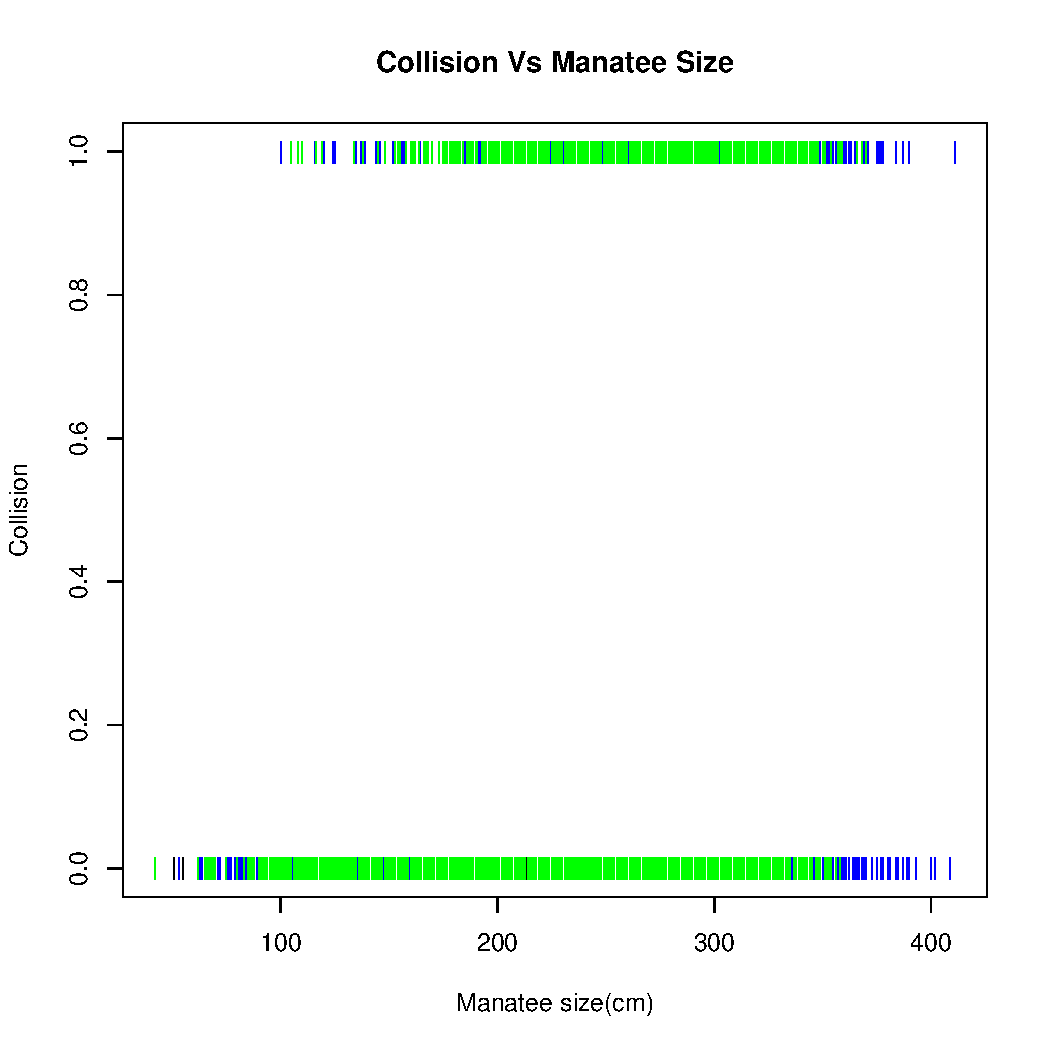
\includegraphics[width=\maxwidth]{figure/unnamed-chunk-14-1} 

\end{knitrout}


\begin{knitrout}
\definecolor{shadecolor}{rgb}{0.969, 0.969, 0.969}\color{fgcolor}\begin{kframe}
\begin{alltt}
\hlstd{wc} \hlkwb{<-} \hlstd{mortDat[mortDat[}\hlstr{'Collision'}\hlstd{]} \hlopt{==} \hlnum{TRUE}\hlstd{, ]}  \hlcom{#Population with collision}
\hlstd{nc} \hlkwb{<-} \hlstd{mortDat[mortDat[}\hlstr{'Collision'}\hlstd{]} \hlopt{==} \hlnum{FALSE}\hlstd{, ]} \hlcom{#Population without collision}

\hlkwd{aggregate}\hlstd{(Collision} \hlopt{~} \hlstd{Season, wc, length)} \hlcom{#Some Evidence of a difference by Season. }
\end{alltt}
\begin{verbatim}
##   Season Collision
## 1   Fall       371
## 2 Spring       660
## 3 Summer       578
## 4 Winter       538
\end{verbatim}
\end{kframe}
\end{knitrout}
Season Visulization
\begin{knitrout}
\definecolor{shadecolor}{rgb}{0.969, 0.969, 0.969}\color{fgcolor}\begin{kframe}
\begin{alltt}
\hlstd{season} \hlkwb{=} \hlstd{wc[}\hlstr{"Season"}\hlstd{]}
\hlstd{season.freq} \hlkwb{=} \hlkwd{table}\hlstd{(season)}
\hlstd{colors} \hlkwb{=} \hlkwd{c}\hlstd{(}\hlstr{"brown"}\hlstd{,} \hlstr{"green"}\hlstd{,} \hlstr{"yellow"}\hlstd{,} \hlstr{"blue"}\hlstd{)}
\hlkwd{barplot}\hlstd{(season.freq,} \hlkwc{col}\hlstd{=colors,}        \hlkwc{legend} \hlstd{=} \hlkwd{rownames}\hlstd{(season.freq),} \hlkwc{main}\hlstd{=}\hlstr{"Number of Collisions "}\hlstd{)}
\end{alltt}
\end{kframe}
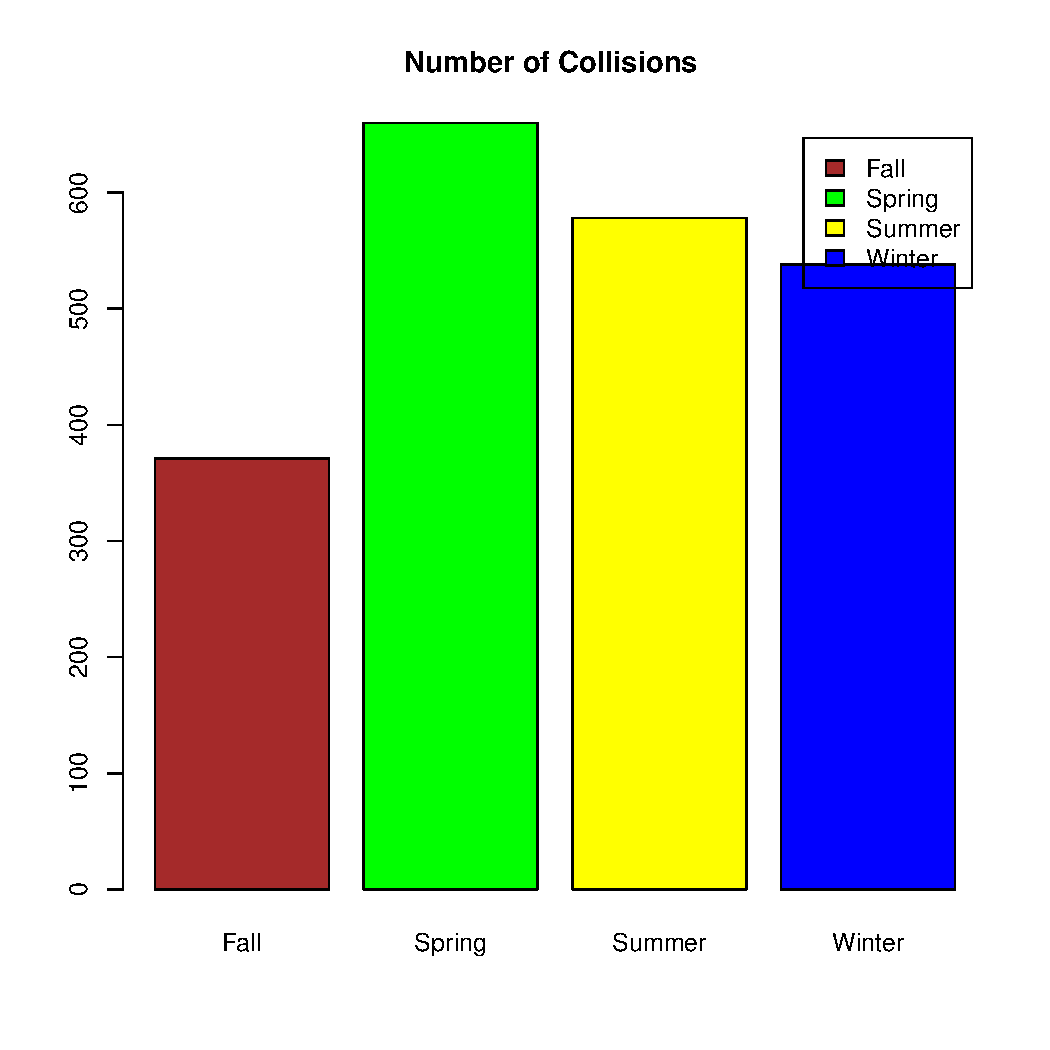
\includegraphics[width=\maxwidth]{figure/unnamed-chunk-16-1} 

\end{knitrout}

\section*{Random sampling based Nonmetric Multidimensional Scaling Code}
\begin{knitrout}
\definecolor{shadecolor}{rgb}{0.969, 0.969, 0.969}\color{fgcolor}\begin{kframe}
\begin{alltt}
\hlkwd{library}\hlstd{(vegan)}
\end{alltt}


{\ttfamily\noindent\itshape\color{messagecolor}{\#\# Loading required package: permute}}

{\ttfamily\noindent\itshape\color{messagecolor}{\#\# Loading required package: lattice}}

{\ttfamily\noindent\itshape\color{messagecolor}{\#\# This is vegan 2.3-4}}\begin{alltt}
\hlstd{alt} \hlkwb{<-} \hlstd{mortDat[}\hlopt{!}\hlstd{(mortDat[}\hlstr{"Sex"}\hlstd{]} \hlopt{==} \hlstr{"U"}\hlstd{),]}
\hlstd{alt} \hlkwb{<-} \hlstd{alt[,}\hlkwd{c}\hlstd{(}\hlstr{"Region"}\hlstd{,} \hlstr{"Sex"}\hlstd{,} \hlstr{"Sizecm"}\hlstd{,} \hlstr{"Season"}\hlstd{,} \hlstr{"Collision"}\hlstd{)]}
\hlstd{altP} \hlkwb{<-} \hlstd{alt[alt}\hlopt{$}\hlstd{Collision} \hlopt{==} \hlnum{TRUE}\hlstd{,} \hlkwd{c}\hlstd{(}\hlstr{"Region"}\hlstd{,} \hlstr{"Sex"}\hlstd{,} \hlstr{"Sizecm"}\hlstd{,} \hlstr{"Season"}\hlstd{,} \hlstr{"Collision"}\hlstd{)]} \hlcom{#Collision population}
\hlstd{altNP} \hlkwb{<-} \hlstd{alt[alt}\hlopt{$}\hlstd{Collision} \hlopt{==} \hlnum{FALSE}\hlstd{,} \hlkwd{c}\hlstd{(}\hlstr{"Region"}\hlstd{,} \hlstr{"Sex"}\hlstd{,} \hlstr{"Sizecm"}\hlstd{,} \hlstr{"Season"}\hlstd{,} \hlstr{"Collision"}\hlstd{)]} \hlcom{#Non-Collision population}
\hlstd{altR} \hlkwb{<-} \hlkwd{rbind}\hlstd{(altP[}\hlkwd{sample}\hlstd{(}\hlnum{1}\hlopt{:}\hlkwd{length}\hlstd{(altP}\hlopt{$}\hlstd{Region),} \hlnum{500}\hlstd{),], altNP[}\hlkwd{sample}\hlstd{(}\hlnum{1}\hlopt{:}\hlkwd{length}\hlstd{(altNP}\hlopt{$}\hlstd{Region),} \hlnum{500}\hlstd{),])}
\end{alltt}
\end{kframe}
\end{knitrout}
New sample set composed of 500 datapoints each from collision and non-collision. 
\begin{knitrout}
\definecolor{shadecolor}{rgb}{0.969, 0.969, 0.969}\color{fgcolor}\begin{kframe}
\begin{alltt}
\hlcom{#Ordinates categorical variables to be numerical factors}
\hlstd{altR}\hlopt{$}\hlstd{Region} \hlkwb{<-} \hlkwd{as.numeric}\hlstd{(}\hlkwd{factor}\hlstd{(altR}\hlopt{$}\hlstd{Region ,} \hlkwc{levels}\hlstd{=}\hlkwd{unique}\hlstd{(alt}\hlopt{$}\hlstd{Region)))}
\hlstd{altR}\hlopt{$}\hlstd{Sex} \hlkwb{<-} \hlkwd{as.numeric}\hlstd{(}\hlkwd{factor}\hlstd{(altR}\hlopt{$}\hlstd{Sex ,} \hlkwc{levels}\hlstd{=}\hlkwd{unique}\hlstd{(alt}\hlopt{$}\hlstd{Sex)))}
\hlstd{altR}\hlopt{$}\hlstd{Season} \hlkwb{<-} \hlkwd{as.numeric}\hlstd{(}\hlkwd{factor}\hlstd{(altR}\hlopt{$}\hlstd{Season ,} \hlkwc{levels}\hlstd{=}\hlkwd{unique}\hlstd{(alt}\hlopt{$}\hlstd{Season)))}
\hlstd{altR}\hlopt{$}\hlstd{Collision} \hlkwb{<-} \hlkwd{as.numeric}\hlstd{(}\hlkwd{factor}\hlstd{(altR}\hlopt{$}\hlstd{Collision ,} \hlkwc{levels}\hlstd{=}\hlkwd{unique}\hlstd{(alt}\hlopt{$}\hlstd{Collision)))}

\hlstd{c.mds} \hlkwb{<-} \hlkwd{metaMDS}\hlstd{(altR[,}\hlnum{1}\hlopt{:}\hlnum{4}\hlstd{],} \hlkwc{zerodist}\hlstd{=}\hlstr{"add"}\hlstd{)}
\end{alltt}
\begin{verbatim}
## Square root transformation
## Wisconsin double standardization
## Zero dissimilarities changed into  4.649836e-05 
## Run 0 stress 0.1911323 
## Run 1 stress 0.195121 
## Run 2 stress 0.1946653 
## Run 3 stress 0.1939209 
## Run 4 stress 0.1957753 
## Run 5 stress 0.1972962 
## Run 6 stress 0.1918791 
## Run 7 stress 0.1920582 
## Run 8 stress 0.1972366 
## Run 9 stress 0.4203234 
## Run 10 stress 0.1925921 
## Run 11 stress 0.1979674 
## Run 12 stress 0.4203559 
## Run 13 stress 0.1967763 
## Run 14 stress 0.1926891 
## Run 15 stress 0.1973116 
## Run 16 stress 0.1939745 
## Run 17 stress 0.2012732 
## Run 18 stress 0.1927304 
## Run 19 stress 0.1933517 
## Run 20 stress 0.1993899
\end{verbatim}
\begin{alltt}
\hlkwd{par}\hlstd{(}\hlkwc{mfcol} \hlstd{=} \hlkwd{c}\hlstd{(}\hlnum{1}\hlstd{,}\hlnum{1}\hlstd{))}
\hlstd{fig} \hlkwb{<-} \hlkwd{ordiplot}\hlstd{(c.mds,} \hlkwc{type} \hlstd{=} \hlstr{"none"}\hlstd{,} \hlkwc{main} \hlstd{=} \hlstr{"NMDS for Collision and Non-Collision Communities"}\hlstd{)}
\hlkwd{points}\hlstd{(fig,} \hlstr{"sites"}\hlstd{,} \hlkwc{pch}\hlstd{=}\hlnum{16}\hlstd{,} \hlkwc{col}\hlstd{=}\hlkwd{c}\hlstd{(}\hlstr{"dodgerblue"}\hlstd{,} \hlstr{"red"}\hlstd{)[altR}\hlopt{$}\hlstd{Collision],} \hlkwc{bg}\hlstd{=}\hlstr{"white"}\hlstd{,} \hlkwc{cex}\hlstd{=}\hlnum{1.1}\hlstd{)}
\hlkwd{ordihull}\hlstd{(c.mds, altR}\hlopt{$}\hlstd{Collision} \hlopt{==} \hlstr{"2"}\hlstd{,} \hlkwc{display} \hlstd{=} \hlstr{"sites"}\hlstd{,} \hlkwc{draw} \hlstd{=} \hlstr{"polygon"}\hlstd{)}
\end{alltt}
\end{kframe}
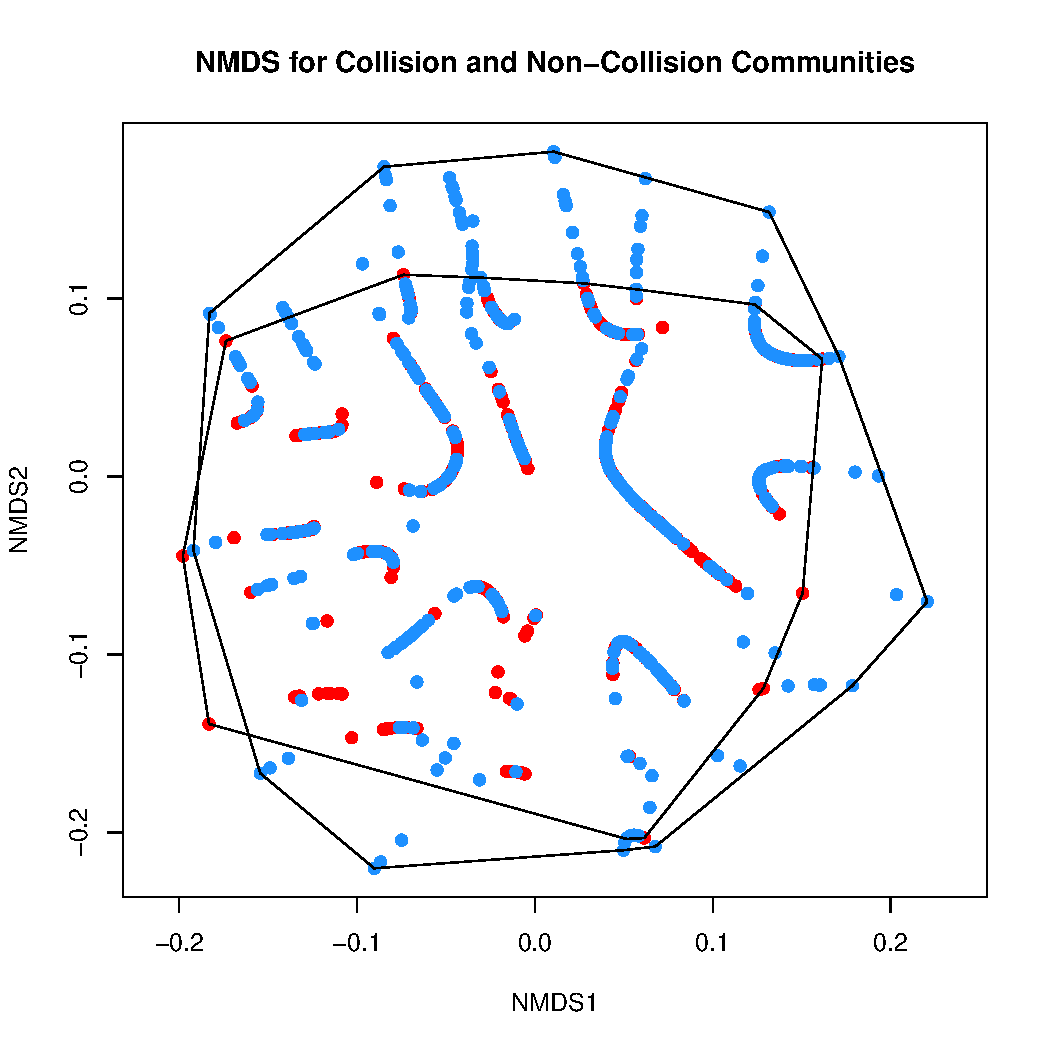
\includegraphics[width=\maxwidth]{figure/unnamed-chunk-18-1} 
\begin{kframe}\begin{alltt}
\hlstd{altR}\hlopt{$}\hlstd{nmds1} \hlkwb{<-} \hlstd{c.mds}\hlopt{$}\hlstd{points[,}\hlnum{1}\hlstd{]}
\hlstd{altR}\hlopt{$}\hlstd{nmds2} \hlkwb{<-} \hlstd{c.mds}\hlopt{$}\hlstd{points[,}\hlnum{2}\hlstd{]}

\hlkwd{pairs}\hlstd{(altR[,}\hlnum{6}\hlopt{:}\hlnum{7}\hlstd{],} \hlkwc{col}\hlstd{=} \hlkwd{c}\hlstd{(}\hlstr{"dodgerblue"}\hlstd{,} \hlstr{"red"}\hlstd{)[altR}\hlopt{$}\hlstd{Collision],} \hlkwc{pch} \hlstd{=} \hlnum{16}\hlstd{,} \hlkwc{main} \hlstd{=} \hlstr{"NMDS for Collision and Non-Collision Communities"}\hlstd{)}
\end{alltt}
\end{kframe}
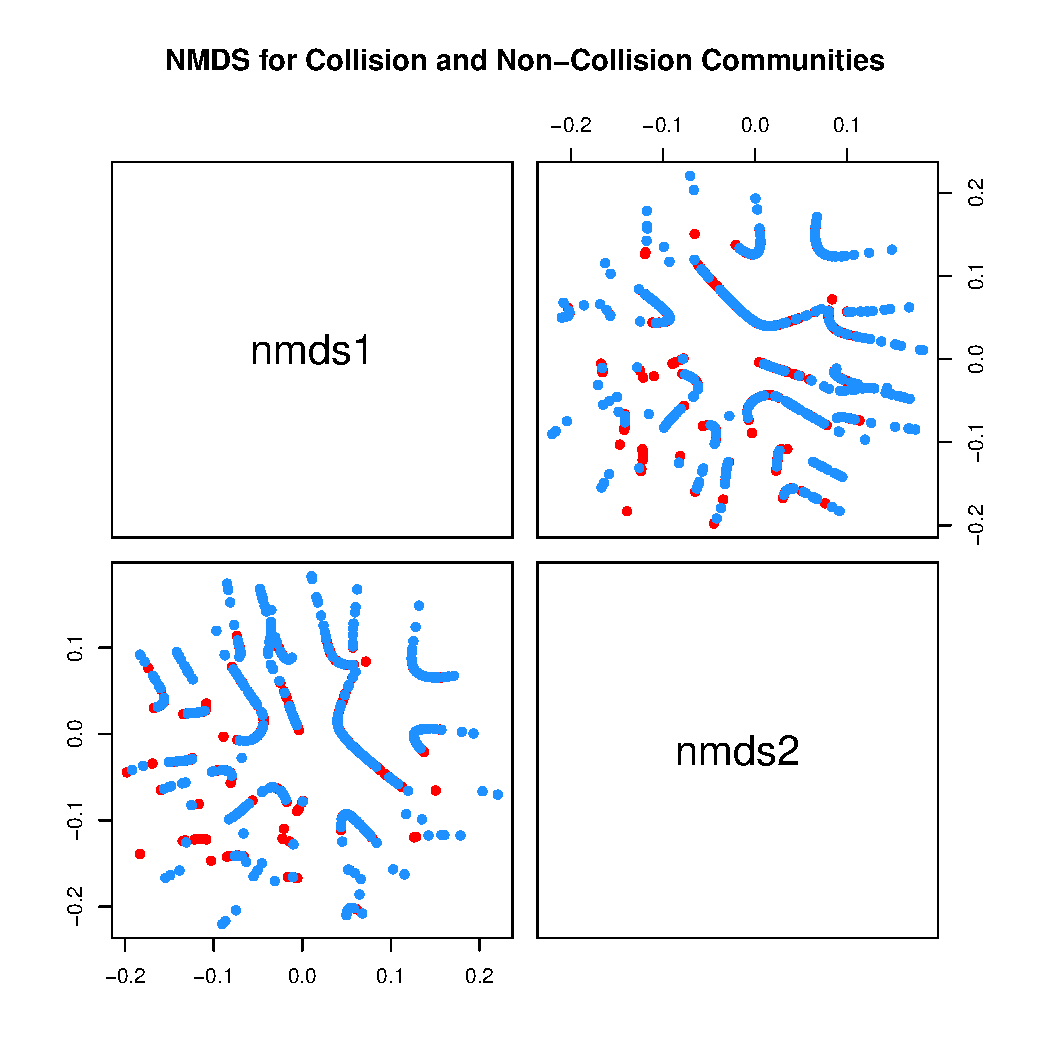
\includegraphics[width=\maxwidth]{figure/unnamed-chunk-18-2} 

\end{knitrout}
\section*{Generalized Linear Modeling Selection Process}

\begin{knitrout}
\definecolor{shadecolor}{rgb}{0.969, 0.969, 0.969}\color{fgcolor}\begin{kframe}
\begin{alltt}
\hlkwd{library}\hlstd{(xtable)}
\hlcom{#Model Selection}

\hlstd{mortD} \hlkwb{<-} \hlstd{mortDat[}\hlopt{!}\hlstd{(mortDat[}\hlstr{"Sex"}\hlstd{]} \hlopt{==} \hlstr{"U"}\hlstd{),]}

\hlkwd{options}\hlstd{(}\hlkwc{na.action} \hlstd{=} \hlstr{"na.fail"}\hlstd{)} \hlcom{#Specifies NA treatment}
\hlstd{subset} \hlkwb{<-} \hlstd{mortD[}\hlkwd{c}\hlstd{(}\hlstr{"Sizecm"}\hlstd{,}\hlstr{"Region"}\hlstd{,} \hlstr{"Sex"}\hlstd{,} \hlstr{"Season"}\hlstd{,}\hlstr{"Collision"}\hlstd{)]} \hlcom{#Subsets data to the explanatory and reposn variables only. }
\hlstd{maximal} \hlkwb{<-} \hlkwd{glm}\hlstd{(Collision} \hlopt{~} \hlstd{Sizecm}\hlopt{*}\hlstd{Region}\hlopt{*}\hlstd{Sex}\hlopt{*}\hlstd{Season,} \hlkwc{data} \hlstd{= subset,} \hlkwc{family} \hlstd{= binomial,} \hlkwc{na.action} \hlstd{= na.fail)}
\end{alltt}
\end{kframe}
\end{knitrout}
\subsection*{STEP AIC Method}
\begin{knitrout}
\definecolor{shadecolor}{rgb}{0.969, 0.969, 0.969}\color{fgcolor}\begin{kframe}
\begin{alltt}
\hlstd{model} \hlkwb{<-} \hlkwd{glm}\hlstd{(Collision} \hlopt{~} \hlstd{Sizecm}\hlopt{*}\hlstd{Region}\hlopt{*}\hlstd{Sex}\hlopt{*}\hlstd{Season,} \hlkwc{data} \hlstd{= mortD,} \hlkwc{family} \hlstd{= binomial,} \hlkwc{na.action} \hlstd{= na.fail)} \hlcom{# Maximal Model}
\hlkwd{summary}\hlstd{(model)}
\end{alltt}
\begin{verbatim}
## 
## Call:
## glm(formula = Collision ~ Sizecm * Region * Sex * Season, family = binomial, 
##     data = mortD, na.action = na.fail)
## 
## Deviance Residuals: 
##     Min       1Q   Median       3Q      Max  
## -1.8715  -0.7261  -0.4646  -0.2902   2.5633  
## 
## Coefficients:
##                                                   Estimate Std. Error
## (Intercept)                                     -3.9792753  1.4904950
## Sizecm                                           0.0105109  0.0053728
## RegionNorthWestCentral                          -1.4770445  4.2154018
## RegionSouthCentralEast                          -0.2374862  1.6135738
## RegionSouthCentralWest                           0.9182840  1.5967759
## SexM                                             1.6645543  1.8710938
## SeasonSpring                                     0.9858437  1.6836772
## SeasonSummer                                     1.2378793  1.6882345
## SeasonWinter                                    -1.5663994  2.2063178
## Sizecm:RegionNorthWestCentral                    0.0091041  0.0167030
## Sizecm:RegionSouthCentralEast                    0.0004921  0.0058147
## Sizecm:RegionSouthCentralWest                   -0.0020174  0.0057789
## Sizecm:SexM                                     -0.0027896  0.0068306
## RegionNorthWestCentral:SexM                     -1.0431218  7.0328503
## RegionSouthCentralEast:SexM                     -2.0036415  2.0626063
## RegionSouthCentralWest:SexM                     -2.5748479  2.0450856
## Sizecm:SeasonSpring                             -0.0006557  0.0060754
## Sizecm:SeasonSummer                             -0.0038117  0.0060281
## Sizecm:SeasonWinter                              0.0033545  0.0081739
## RegionNorthWestCentral:SeasonSpring              1.3086386  4.5601541
## RegionSouthCentralEast:SeasonSpring             -1.0267916  1.8505785
## RegionSouthCentralWest:SeasonSpring             -0.9823429  1.8132461
## RegionNorthWestCentral:SeasonSummer              0.7322562  5.2893006
## RegionSouthCentralEast:SeasonSummer             -0.9318533  1.8636635
## RegionSouthCentralWest:SeasonSummer             -1.7804699  1.8348033
## RegionNorthWestCentral:SeasonWinter              1.5541247  6.3392272
## RegionSouthCentralEast:SeasonWinter              1.2099843  2.3350573
## RegionSouthCentralWest:SeasonWinter              0.3312152  2.3322402
## SexM:SeasonSpring                               -6.2511615  2.4824137
## SexM:SeasonSummer                               -3.6821017  2.2920365
## SexM:SeasonWinter                               -0.6042932  3.0577212
## Sizecm:RegionNorthWestCentral:SexM              -0.0035674  0.0254683
## Sizecm:RegionSouthCentralEast:SexM               0.0053262  0.0075449
## Sizecm:RegionSouthCentralWest:SexM               0.0062116  0.0075196
## Sizecm:RegionNorthWestCentral:SeasonSpring      -0.0128531  0.0179025
## Sizecm:RegionSouthCentralEast:SeasonSpring       0.0022954  0.0066838
## Sizecm:RegionSouthCentralWest:SeasonSpring       0.0011069  0.0065784
## Sizecm:RegionNorthWestCentral:SeasonSummer      -0.0107289  0.0205092
## Sizecm:RegionSouthCentralEast:SeasonSummer       0.0032662  0.0066546
## Sizecm:RegionSouthCentralWest:SeasonSummer       0.0074382  0.0065887
## Sizecm:RegionNorthWestCentral:SeasonWinter      -0.0098543  0.0266129
## Sizecm:RegionSouthCentralEast:SeasonWinter      -0.0021934  0.0086336
## Sizecm:RegionSouthCentralWest:SeasonWinter      -0.0016841  0.0086384
## Sizecm:SexM:SeasonSpring                         0.0210785  0.0089779
## Sizecm:SexM:SeasonSummer                         0.0134853  0.0083013
## Sizecm:SexM:SeasonWinter                        -0.0022245  0.0115304
## RegionNorthWestCentral:SexM:SeasonSpring         2.5499119  7.6373634
## RegionSouthCentralEast:SexM:SeasonSpring         6.2649663  2.7052993
## RegionSouthCentralWest:SexM:SeasonSpring         6.3158963  2.6766517
## RegionNorthWestCentral:SexM:SeasonSummer         2.8314487  8.2198145
## RegionSouthCentralEast:SexM:SeasonSummer         3.2718067  2.5471781
## RegionSouthCentralWest:SexM:SeasonSummer         3.1578815  2.5416806
## RegionNorthWestCentral:SexM:SeasonWinter         1.6978567  9.5858797
## RegionSouthCentralEast:SexM:SeasonWinter         0.9962753  3.2440849
## RegionSouthCentralWest:SexM:SeasonWinter         1.5897948  3.2494577
## Sizecm:RegionNorthWestCentral:SexM:SeasonSpring  0.0031795  0.0279352
## Sizecm:RegionSouthCentralEast:SexM:SeasonSpring -0.0219140  0.0098254
## Sizecm:RegionSouthCentralWest:SexM:SeasonSpring -0.0224944  0.0097599
## Sizecm:RegionNorthWestCentral:SexM:SeasonSummer -0.0007464  0.0299511
## Sizecm:RegionSouthCentralEast:SexM:SeasonSummer -0.0109615  0.0092528
## Sizecm:RegionSouthCentralWest:SexM:SeasonSummer -0.0105737  0.0093010
## Sizecm:RegionNorthWestCentral:SexM:SeasonWinter -0.0023414  0.0370964
## Sizecm:RegionSouthCentralEast:SexM:SeasonWinter -0.0003113  0.0122189
## Sizecm:RegionSouthCentralWest:SexM:SeasonWinter -0.0016075  0.0122604
##                                                 z value Pr(>|z|)   
## (Intercept)                                      -2.670  0.00759 **
## Sizecm                                            1.956  0.05043 . 
## RegionNorthWestCentral                           -0.350  0.72604   
## RegionSouthCentralEast                           -0.147  0.88299   
## RegionSouthCentralWest                            0.575  0.56523   
## SexM                                              0.890  0.37367   
## SeasonSpring                                      0.586  0.55819   
## SeasonSummer                                      0.733  0.46341   
## SeasonWinter                                     -0.710  0.47773   
## Sizecm:RegionNorthWestCentral                     0.545  0.58571   
## Sizecm:RegionSouthCentralEast                     0.085  0.93255   
## Sizecm:RegionSouthCentralWest                    -0.349  0.72702   
## Sizecm:SexM                                      -0.408  0.68298   
## RegionNorthWestCentral:SexM                      -0.148  0.88209   
## RegionSouthCentralEast:SexM                      -0.971  0.33134   
## RegionSouthCentralWest:SexM                      -1.259  0.20802   
## Sizecm:SeasonSpring                              -0.108  0.91405   
## Sizecm:SeasonSummer                              -0.632  0.52718   
## Sizecm:SeasonWinter                               0.410  0.68152   
## RegionNorthWestCentral:SeasonSpring               0.287  0.77413   
## RegionSouthCentralEast:SeasonSpring              -0.555  0.57900   
## RegionSouthCentralWest:SeasonSpring              -0.542  0.58798   
## RegionNorthWestCentral:SeasonSummer               0.138  0.88989   
## RegionSouthCentralEast:SeasonSummer              -0.500  0.61707   
## RegionSouthCentralWest:SeasonSummer              -0.970  0.33185   
## RegionNorthWestCentral:SeasonWinter               0.245  0.80633   
## RegionSouthCentralEast:SeasonWinter               0.518  0.60433   
## RegionSouthCentralWest:SeasonWinter               0.142  0.88707   
## SexM:SeasonSpring                                -2.518  0.01180 * 
## SexM:SeasonSummer                                -1.606  0.10817   
## SexM:SeasonWinter                                -0.198  0.84334   
## Sizecm:RegionNorthWestCentral:SexM               -0.140  0.88860   
## Sizecm:RegionSouthCentralEast:SexM                0.706  0.48023   
## Sizecm:RegionSouthCentralWest:SexM                0.826  0.40877   
## Sizecm:RegionNorthWestCentral:SeasonSpring       -0.718  0.47279   
## Sizecm:RegionSouthCentralEast:SeasonSpring        0.343  0.73128   
## Sizecm:RegionSouthCentralWest:SeasonSpring        0.168  0.86638   
## Sizecm:RegionNorthWestCentral:SeasonSummer       -0.523  0.60089   
## Sizecm:RegionSouthCentralEast:SeasonSummer        0.491  0.62356   
## Sizecm:RegionSouthCentralWest:SeasonSummer        1.129  0.25892   
## Sizecm:RegionNorthWestCentral:SeasonWinter       -0.370  0.71117   
## Sizecm:RegionSouthCentralEast:SeasonWinter       -0.254  0.79946   
## Sizecm:RegionSouthCentralWest:SeasonWinter       -0.195  0.84543   
## Sizecm:SexM:SeasonSpring                          2.348  0.01888 * 
## Sizecm:SexM:SeasonSummer                          1.624  0.10428   
## Sizecm:SexM:SeasonWinter                         -0.193  0.84702   
## RegionNorthWestCentral:SexM:SeasonSpring          0.334  0.73848   
## RegionSouthCentralEast:SexM:SeasonSpring          2.316  0.02057 * 
## RegionSouthCentralWest:SexM:SeasonSpring          2.360  0.01829 * 
## RegionNorthWestCentral:SexM:SeasonSummer          0.344  0.73050   
## RegionSouthCentralEast:SexM:SeasonSummer          1.284  0.19897   
## RegionSouthCentralWest:SexM:SeasonSummer          1.242  0.21407   
## RegionNorthWestCentral:SexM:SeasonWinter          0.177  0.85941   
## RegionSouthCentralEast:SexM:SeasonWinter          0.307  0.75876   
## RegionSouthCentralWest:SexM:SeasonWinter          0.489  0.62467   
## Sizecm:RegionNorthWestCentral:SexM:SeasonSpring   0.114  0.90938   
## Sizecm:RegionSouthCentralEast:SexM:SeasonSpring  -2.230  0.02572 * 
## Sizecm:RegionSouthCentralWest:SexM:SeasonSpring  -2.305  0.02118 * 
## Sizecm:RegionNorthWestCentral:SexM:SeasonSummer  -0.025  0.98012   
## Sizecm:RegionSouthCentralEast:SexM:SeasonSummer  -1.185  0.23615   
## Sizecm:RegionSouthCentralWest:SexM:SeasonSummer  -1.137  0.25561   
## Sizecm:RegionNorthWestCentral:SexM:SeasonWinter  -0.063  0.94967   
## Sizecm:RegionSouthCentralEast:SexM:SeasonWinter  -0.025  0.97968   
## Sizecm:RegionSouthCentralWest:SexM:SeasonWinter  -0.131  0.89569   
## ---
## Signif. codes:  0 '***' 0.001 '**' 0.01 '*' 0.05 '.' 0.1 ' ' 1
## 
## (Dispersion parameter for binomial family taken to be 1)
## 
##     Null deviance: 10122.5  on 9506  degrees of freedom
## Residual deviance:  8778.3  on 9443  degrees of freedom
## AIC: 8906.3
## 
## Number of Fisher Scoring iterations: 5
\end{verbatim}
\begin{alltt}
\hlstd{model2} \hlkwb{<-} \hlkwd{step}\hlstd{(model)} \hlcom{#Step AIC model reduction }
\end{alltt}
\begin{verbatim}
## Start:  AIC=8906.29
## Collision ~ Sizecm * Region * Sex * Season
## 
##                            Df Deviance    AIC
## - Sizecm:Region:Sex:Season  9   8787.5 8897.5
## <none>                          8778.3 8906.3
## 
## Step:  AIC=8897.54
## Collision ~ Sizecm + Region + Sex + Season + Sizecm:Region + 
##     Sizecm:Sex + Region:Sex + Sizecm:Season + Region:Season + 
##     Sex:Season + Sizecm:Region:Sex + Sizecm:Region:Season + Sizecm:Sex:Season + 
##     Region:Sex:Season
## 
##                        Df Deviance    AIC
## - Region:Sex:Season     9   8796.4 8888.4
## - Sizecm:Region:Season  9   8800.5 8892.5
## - Sizecm:Region:Sex     3   8791.7 8895.7
## <none>                      8787.5 8897.5
## - Sizecm:Sex:Season     3   8793.8 8897.8
## 
## Step:  AIC=8888.39
## Collision ~ Sizecm + Region + Sex + Season + Sizecm:Region + 
##     Sizecm:Sex + Region:Sex + Sizecm:Season + Region:Season + 
##     Sex:Season + Sizecm:Region:Sex + Sizecm:Region:Season + Sizecm:Sex:Season
## 
##                        Df Deviance    AIC
## - Sizecm:Region:Season  9   8809.3 8883.3
## - Sizecm:Region:Sex     3   8800.5 8886.5
## <none>                      8796.4 8888.4
## - Sizecm:Sex:Season     3   8802.6 8888.6
## 
## Step:  AIC=8883.28
## Collision ~ Sizecm + Region + Sex + Season + Sizecm:Region + 
##     Sizecm:Sex + Region:Sex + Sizecm:Season + Region:Season + 
##     Sex:Season + Sizecm:Region:Sex + Sizecm:Sex:Season
## 
##                     Df Deviance    AIC
## - Sizecm:Region:Sex  3   8813.7 8881.7
## - Sizecm:Sex:Season  3   8815.1 8883.1
## <none>                   8809.3 8883.3
## - Region:Season      9   8870.9 8926.9
## 
## Step:  AIC=8881.75
## Collision ~ Sizecm + Region + Sex + Season + Sizecm:Region + 
##     Sizecm:Sex + Region:Sex + Sizecm:Season + Region:Season + 
##     Sex:Season + Sizecm:Sex:Season
## 
##                     Df Deviance    AIC
## - Sizecm:Region      3   8816.7 8878.7
## <none>                   8813.7 8881.7
## - Sizecm:Sex:Season  3   8820.9 8882.9
## - Region:Sex         3   8825.6 8887.6
## - Region:Season      9   8875.5 8925.5
## 
## Step:  AIC=8878.72
## Collision ~ Sizecm + Region + Sex + Season + Sizecm:Sex + Region:Sex + 
##     Sizecm:Season + Region:Season + Sex:Season + Sizecm:Sex:Season
## 
##                     Df Deviance    AIC
## <none>                   8816.7 8878.7
## - Sizecm:Sex:Season  3   8824.1 8880.1
## - Region:Sex         3   8827.9 8883.9
## - Region:Season      9   8878.7 8922.7
\end{verbatim}
\begin{alltt}
\hlkwd{summary}\hlstd{(model2)}
\end{alltt}
\begin{verbatim}
## 
## Call:
## glm(formula = Collision ~ Sizecm + Region + Sex + Season + Sizecm:Sex + 
##     Region:Sex + Sizecm:Season + Region:Season + Sex:Season + 
##     Sizecm:Sex:Season, family = binomial, data = mortD, na.action = na.fail)
## 
## Deviance Residuals: 
##     Min       1Q   Median       3Q      Max  
## -1.7406  -0.7283  -0.4632  -0.2910   2.7645  
## 
## Coefficients:
##                                       Estimate Std. Error z value Pr(>|z|)
## (Intercept)                         -3.5588986  0.4598964  -7.738 1.01e-14
## Sizecm                               0.0098506  0.0014597   6.748 1.50e-11
## RegionNorthWestCentral              -0.6669296  0.7127040  -0.936 0.349390
## RegionSouthCentralEast              -0.3498613  0.2639951  -1.325 0.185086
## RegionSouthCentralWest               0.1258460  0.2587647   0.486 0.626731
## SexM                                -0.0807929  0.5870742  -0.138 0.890541
## SeasonSpring                         0.4529067  0.5386926   0.841 0.400487
## SeasonSummer                        -0.2445034  0.5647746  -0.433 0.665071
## SeasonWinter                        -1.6186623  0.5857172  -2.764 0.005718
## Sizecm:SexM                          0.0022902  0.0021008   1.090 0.275643
## RegionNorthWestCentral:SexM          0.1580309  0.5725747   0.276 0.782548
## RegionSouthCentralEast:SexM         -0.2081688  0.1938159  -1.074 0.282798
## RegionSouthCentralWest:SexM         -0.4996420  0.1927597  -2.592 0.009541
## Sizecm:SeasonSpring                  0.0004482  0.0017497   0.256 0.797839
## Sizecm:SeasonSummer                  0.0007891  0.0018095   0.436 0.662758
## Sizecm:SeasonWinter                  0.0013904  0.0018874   0.737 0.461330
## RegionNorthWestCentral:SeasonSpring -0.0543141  0.6962555  -0.078 0.937821
## RegionSouthCentralEast:SeasonSpring -0.1620992  0.2923679  -0.554 0.579281
## RegionSouthCentralWest:SeasonSpring -0.4580531  0.2867128  -1.598 0.110131
## RegionNorthWestCentral:SeasonSummer -0.1862646  0.8483267  -0.220 0.826208
## RegionSouthCentralEast:SeasonSummer  0.2058133  0.2985816   0.689 0.490632
## RegionSouthCentralWest:SeasonSummer  0.4360056  0.2940571   1.483 0.138148
## RegionNorthWestCentral:SeasonWinter -0.4387200  0.8339371  -0.526 0.598831
## RegionSouthCentralEast:SeasonWinter  1.1658173  0.3178515   3.668 0.000245
## RegionSouthCentralWest:SeasonWinter  0.5518911  0.3168227   1.742 0.081516
## SexM:SeasonSpring                   -0.7388077  0.6850617  -1.078 0.280831
## SexM:SeasonSummer                   -0.7798668  0.7235299  -1.078 0.281094
## SexM:SeasonWinter                    0.4416666  0.7329603   0.603 0.546789
## Sizecm:SexM:SeasonSpring             0.0018851  0.0025771   0.731 0.464478
## Sizecm:SexM:SeasonSummer             0.0039181  0.0027047   1.449 0.147443
## Sizecm:SexM:SeasonWinter            -0.0024947  0.0027598  -0.904 0.366013
##                                        
## (Intercept)                         ***
## Sizecm                              ***
## RegionNorthWestCentral                 
## RegionSouthCentralEast                 
## RegionSouthCentralWest                 
## SexM                                   
## SeasonSpring                           
## SeasonSummer                           
## SeasonWinter                        ** 
## Sizecm:SexM                            
## RegionNorthWestCentral:SexM            
## RegionSouthCentralEast:SexM            
## RegionSouthCentralWest:SexM         ** 
## Sizecm:SeasonSpring                    
## Sizecm:SeasonSummer                    
## Sizecm:SeasonWinter                    
## RegionNorthWestCentral:SeasonSpring    
## RegionSouthCentralEast:SeasonSpring    
## RegionSouthCentralWest:SeasonSpring    
## RegionNorthWestCentral:SeasonSummer    
## RegionSouthCentralEast:SeasonSummer    
## RegionSouthCentralWest:SeasonSummer    
## RegionNorthWestCentral:SeasonWinter    
## RegionSouthCentralEast:SeasonWinter ***
## RegionSouthCentralWest:SeasonWinter .  
## SexM:SeasonSpring                      
## SexM:SeasonSummer                      
## SexM:SeasonWinter                      
## Sizecm:SexM:SeasonSpring               
## Sizecm:SexM:SeasonSummer               
## Sizecm:SexM:SeasonWinter               
## ---
## Signif. codes:  0 '***' 0.001 '**' 0.01 '*' 0.05 '.' 0.1 ' ' 1
## 
## (Dispersion parameter for binomial family taken to be 1)
## 
##     Null deviance: 10122.5  on 9506  degrees of freedom
## Residual deviance:  8816.7  on 9476  degrees of freedom
## AIC: 8878.7
## 
## Number of Fisher Scoring iterations: 5
\end{verbatim}
\end{kframe}
\end{knitrout}
\subsection*{Resulting models}
\begin{knitrout}
\definecolor{shadecolor}{rgb}{0.969, 0.969, 0.969}\color{fgcolor}\begin{kframe}
\begin{alltt}
\hlstd{stepAICModel} \hlkwb{<-} \hlkwd{glm}\hlstd{(}\hlkwc{formula} \hlstd{= Collision} \hlopt{~} \hlstd{Sizecm} \hlopt{+} \hlstd{Region} \hlopt{+} \hlstd{Sex} \hlopt{+} \hlstd{Season} \hlopt{+} \hlstd{Sizecm}\hlopt{:}\hlstd{Sex} \hlopt{+}
      \hlstd{Region}\hlopt{:}\hlstd{Sex} \hlopt{+} \hlstd{Sizecm}\hlopt{:}\hlstd{Season} \hlopt{+} \hlstd{Region}\hlopt{:}\hlstd{Season} \hlopt{+} \hlstd{Sex}\hlopt{:}\hlstd{Season} \hlopt{+}
      \hlstd{Sizecm}\hlopt{:}\hlstd{Sex}\hlopt{:}\hlstd{Season,} \hlkwc{family} \hlstd{= binomial,} \hlkwc{data} \hlstd{= mortD,} \hlkwc{na.action} \hlstd{= na.fail)}
\end{alltt}
\end{kframe}
\end{knitrout}
Step AIC Reduced Model
\begin{knitrout}
\definecolor{shadecolor}{rgb}{0.969, 0.969, 0.969}\color{fgcolor}\begin{kframe}
\begin{alltt}
\hlstd{oneStep}  \hlkwb{<-} \hlkwd{glm}\hlstd{(}\hlkwc{formula} \hlstd{= Collision} \hlopt{~} \hlstd{Sizecm} \hlopt{+} \hlstd{Region} \hlopt{+} \hlstd{Sex} \hlopt{+} \hlstd{Season} \hlopt{+} \hlstd{Sizecm}\hlopt{:}\hlstd{Sex} \hlopt{+}
                  \hlstd{Region}\hlopt{:}\hlstd{Sex} \hlopt{+} \hlstd{Region}\hlopt{:}\hlstd{Season} \hlopt{+} \hlstd{Sex}\hlopt{:}\hlstd{Season} \hlopt{+}
                  \hlstd{Sizecm}\hlopt{:}\hlstd{Sex}\hlopt{:}\hlstd{Season,} \hlkwc{family} \hlstd{= binomial,} \hlkwc{data} \hlstd{= mortD,} \hlkwc{na.action} \hlstd{= na.fail)}
\end{alltt}
\end{kframe}
\end{knitrout}
Removal of Sex:Season in comparison to StepAIC model
\begin{knitrout}
\definecolor{shadecolor}{rgb}{0.969, 0.969, 0.969}\color{fgcolor}\begin{kframe}
\begin{alltt}
\hlstd{oneStepAlt} \hlkwb{<-} \hlkwd{glm}\hlstd{(}\hlkwc{formula} \hlstd{= Collision} \hlopt{~} \hlstd{Sizecm} \hlopt{+} \hlstd{Region} \hlopt{+} \hlstd{Sex} \hlopt{+} \hlstd{Season} \hlopt{+} \hlstd{Sizecm}\hlopt{:}\hlstd{Sex} \hlopt{+}
                  \hlstd{Region}\hlopt{:}\hlstd{Sex} \hlopt{+} \hlstd{Sizecm}\hlopt{:}\hlstd{Season} \hlopt{+} \hlstd{Region}\hlopt{:}\hlstd{Season} \hlopt{+} \hlstd{Sex}\hlopt{:}\hlstd{Season ,}
                  \hlkwc{family} \hlstd{= binomial,} \hlkwc{data} \hlstd{= mortD,} \hlkwc{na.action} \hlstd{= na.fail)}
\end{alltt}
\end{kframe}
\end{knitrout}
Removal of Sizecm:Sex:Season in comparison to StepAIC model

\subsection*{Dredge Model}
\begin{knitrout}
\definecolor{shadecolor}{rgb}{0.969, 0.969, 0.969}\color{fgcolor}\begin{kframe}
\begin{alltt}
\hlkwd{library}\hlstd{(MuMIn)}
\hlstd{dd} \hlkwb{<-} \hlkwd{dredge}\hlstd{(maximal)}
\end{alltt}


{\ttfamily\noindent\itshape\color{messagecolor}{\#\# Fixed term is "{}(Intercept)"{}}}\end{kframe}
\end{knitrout}
Produces model selection table based on AIC ranking from low to high by recursively making all model combinations from the largest possible model. 
\begin{knitrout}
\definecolor{shadecolor}{rgb}{0.969, 0.969, 0.969}\color{fgcolor}\begin{kframe}
\begin{alltt}
\hlstd{dredgeModel} \hlkwb{<-} \hlkwd{glm}\hlstd{(Collision} \hlopt{~} \hlstd{Region} \hlopt{+} \hlstd{Season} \hlopt{+} \hlstd{Sex} \hlopt{+} \hlstd{Sizecm} \hlopt{+} \hlstd{Region}\hlopt{:}\hlstd{Season} \hlopt{+} \hlstd{Region}\hlopt{:}\hlstd{Sex} \hlopt{+} \hlstd{Season}\hlopt{:}\hlstd{Sex} \hlopt{+} \hlstd{Sex}\hlopt{:}\hlstd{Sizecm,} \hlkwc{data} \hlstd{= mortD,} \hlkwc{family} \hlstd{= binomial,} \hlkwc{na.action} \hlstd{= na.fail)}
\hlstd{maximal} \hlkwb{<-} \hlkwd{glm}\hlstd{(Collision} \hlopt{~} \hlstd{Sizecm}\hlopt{*}\hlstd{Region}\hlopt{*}\hlstd{Sex}\hlopt{*}\hlstd{Season,} \hlkwc{data} \hlstd{= subset,} \hlkwc{family} \hlstd{= binomial,} \hlkwc{na.action} \hlstd{= na.fail)}
\end{alltt}
\end{kframe}
\end{knitrout}
\section*{Anova Table Generation}

\begin{knitrout}
\definecolor{shadecolor}{rgb}{0.969, 0.969, 0.969}\color{fgcolor}\begin{kframe}
\begin{alltt}
\hlcom{#Anova Table Generation Code. }

\hlkwd{print}\hlstd{(}\hlkwd{xtable}\hlstd{(}\hlkwd{anova}\hlstd{(maximal, stepAICModel,} \hlkwc{test}\hlstd{=}\hlstr{"Chi"}\hlstd{)))} \hlcom{#Anova Table for maximal model vs Dredge model. }
\end{alltt}
\begin{verbatim}
## % latex table generated in R 3.2.3 by xtable 1.8-2 package
## % Mon Mar 14 01:42:14 2016
## \begin{table}[ht]
## \centering
## \begin{tabular}{lrrrrr}
##   \hline
##  & Resid. Df & Resid. Dev & Df & Deviance & Pr($>$Chi) \\ 
##   \hline
## 1 & 9443 & 8778.29 &  &  &  \\ 
##   2 & 9476 & 8816.72 & -33 & -38.43 & 0.2369 \\ 
##    \hline
## \end{tabular}
## \end{table}
\end{verbatim}
\begin{alltt}
\hlkwd{print}\hlstd{(}\hlkwd{xtable}\hlstd{(}\hlkwd{anova}\hlstd{(maximal, dredgeModel,} \hlkwc{test}\hlstd{=}\hlstr{"Chi"}\hlstd{)))} \hlcom{#Anova Table for maximal model vs Dredge model. }
\end{alltt}
\begin{verbatim}
## % latex table generated in R 3.2.3 by xtable 1.8-2 package
## % Mon Mar 14 01:42:14 2016
## \begin{table}[ht]
## \centering
## \begin{tabular}{lrrrrr}
##   \hline
##  & Resid. Df & Resid. Dev & Df & Deviance & Pr($>$Chi) \\ 
##   \hline
## 1 & 9443 & 8778.29 &  &  &  \\ 
##   2 & 9482 & 8828.62 & -39 & -50.33 & 0.1056 \\ 
##    \hline
## \end{tabular}
## \end{table}
\end{verbatim}
\begin{alltt}
\hlkwd{print}\hlstd{(}\hlkwd{xtable}\hlstd{(}\hlkwd{anova}\hlstd{(maximal, oneStep, oneStepAlt, dredgeModel,} \hlkwc{test}\hlstd{=}\hlstr{"Chi"}\hlstd{)))} \hlcom{#Anova Table for building down from maximal to AICmodel to dredge model.  }
\end{alltt}
\begin{verbatim}
## % latex table generated in R 3.2.3 by xtable 1.8-2 package
## % Mon Mar 14 01:42:14 2016
## \begin{table}[ht]
## \centering
## \begin{tabular}{lrrrrr}
##   \hline
##  & Resid. Df & Resid. Dev & Df & Deviance & Pr($>$Chi) \\ 
##   \hline
## 1 & 9443 & 8778.29 &  &  &  \\ 
##   2 & 9476 & 8816.72 & -33 & -38.43 & 0.2369 \\ 
##   3 & 9479 & 8824.05 & -3 & -7.33 & 0.0622 \\ 
##   4 & 9482 & 8828.62 & -3 & -4.57 & 0.2059 \\ 
##    \hline
## \end{tabular}
## \end{table}
\end{verbatim}
\end{kframe}
\end{knitrout}
\end{document}
